\section{Preliminary Results}

\subsection{Placement changes latency on real hardware}

\begin{table}[t]
\caption{Cluster pilots. Transaction latency with primary copies gathered in
the region issuing the transactions, against spread across regions.}
\label{tab:cluster}
\centering
\footnotesize
\begin{tabular}{llrrr}
\toprule
Pilot & Placement & p50 (ms) & p95 (ms) & stdev (ms) \\
\midrule
$N=200$, 2 cores  & co-located &  272.7 &  275.5 &  48.8 \\
                  & spread     & 1013.4 & 1648.0 & 302.0 \\
\addlinespace
$N=1000$, 4 cores & co-located &  441.5 &  446.6 &  78.4 \\
                  & spread     & 1015.3 & 1648.7 & 299.9 \\
\bottomrule
\end{tabular}
\end{table}

Table~\ref{tab:cluster} reports two pilots in which the same transactions run
twice, once with the primary copies gathered in the region issuing them and
once with them spread across regions. The difference in 95th percentile
latency is 1372.5\,ms in the first pilot and 1202.0\,ms in the second.
Placement is worth a great deal on real hardware, which is the assumption
everything else rests on.

Three qualifications belong with that number. First, co-located means the
primary copies, not the data. With three copies and one node per region the
copies always span three regions, so every write still pays a cross-region
agreement even in the co-located case, which is why that median is 272.7\,ms
rather than single digits. The experiment isolates the effect of where the
primary sits, which is what \textsc{move\_lease} controls.

Second, the figures are indicative rather than precise. At 200 transactions
the 95th percentile is the 190th value in the sorted list, so an interval
around it is unreliable. The second pilot raised the count to 1000 and halved
the interval width from 155.2 to 65.6\,ms.

Third, the co-located case became 62\% slower when the pilot moved from two
cores to four, whilst the spread case barely moved. The hardware and the
transaction count changed together, so this isolates no cause. It is
consistent with every primary landing on one node and that node becoming the
limit, which the simulator cannot reproduce, and it is why imbalance is
charged for separately in~\eqref{eq:objective}.

\subsection{How the room for a better policy changes}

\begin{table}[t]
\caption{Volatility sweep. Mean latency in milliseconds and gigabytes moved
per episode, eight seeds per value, seed block 0 to 7.}
\label{tab:sweep}
\centering
\footnotesize
\begin{tabular}{lrrrrr}
\toprule
Volatility & Fixed & Random & Follow & Reference & Follow GB \\
\midrule
0.5 & 156.27 & 156.79 &  94.31 & 93.87 &  405.1 \\
1.0 & 156.11 & 158.02 &  98.66 & 93.66 &  785.2 \\
2.0 & 155.37 & 158.89 & 125.37 & 89.47 & 1056.6 \\
4.0 & 155.77 & 160.24 & 139.58 & 82.38 & 1115.2 \\
\bottomrule
\end{tabular}
\end{table}

\begin{figure}[t]
\centering
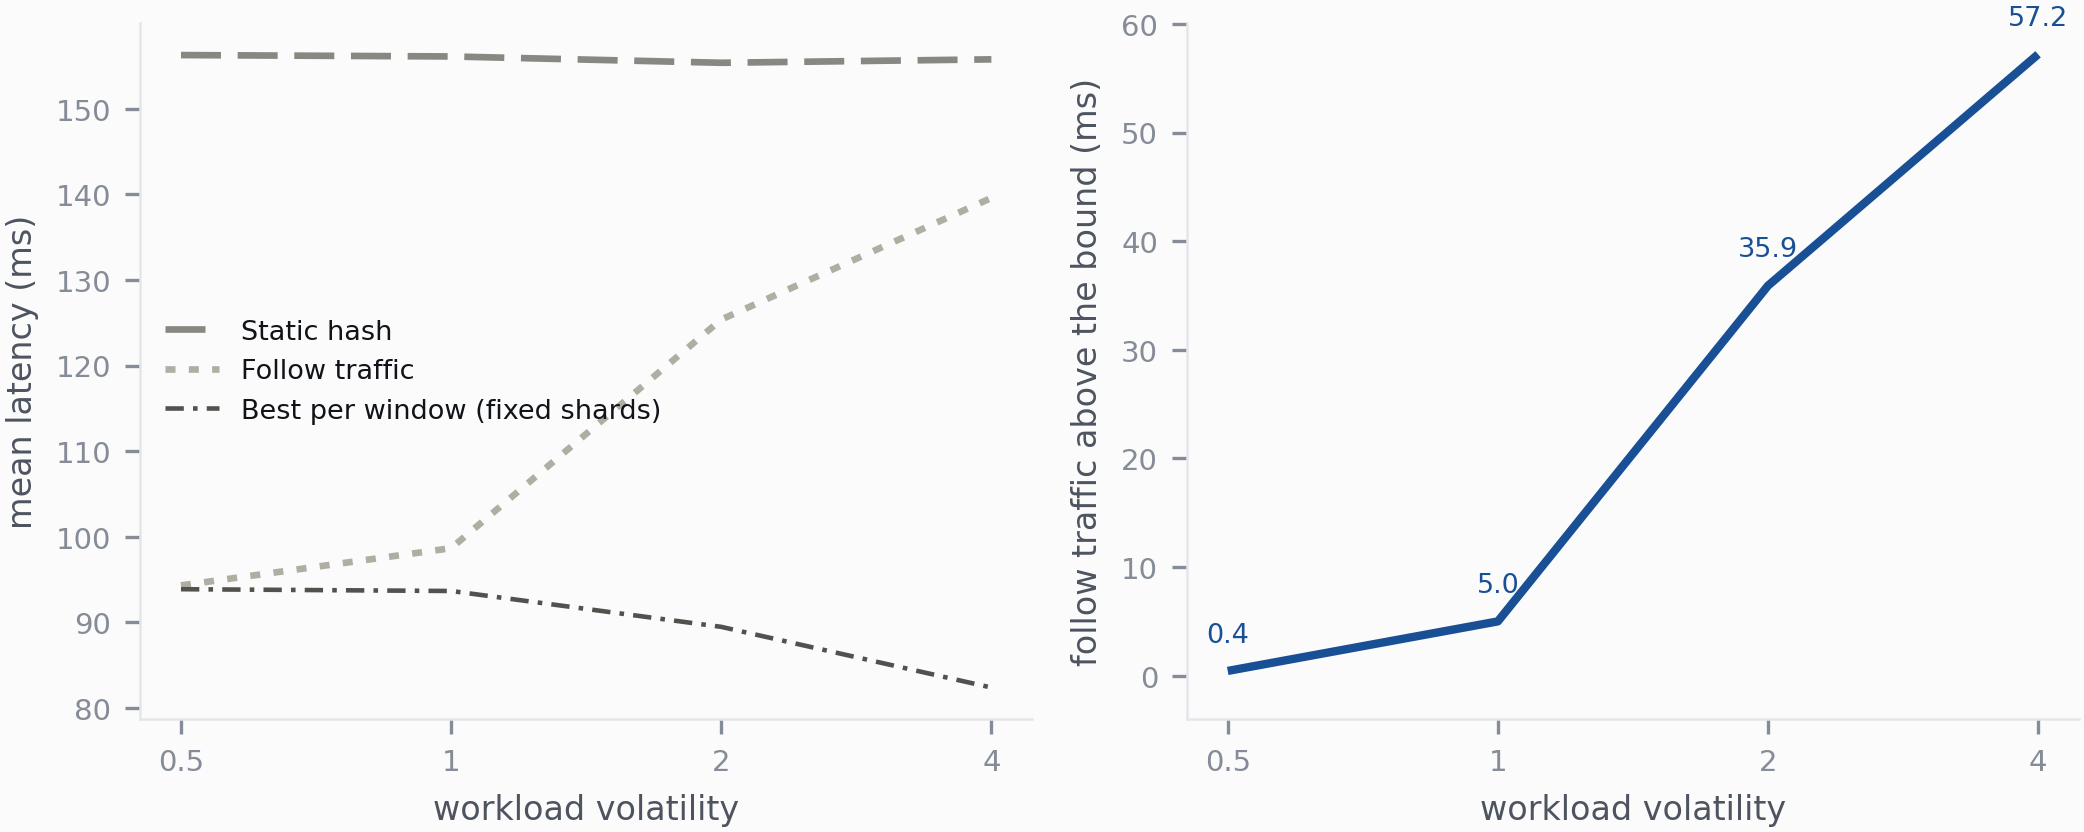
\includegraphics[width=\columnwidth]{sweep.png}
\caption{Left: latency as the traffic moves faster, for fixed placement, the
follow traffic rule, and the cost-free reference. Right: how far the rule sits
above that reference. That distance is the room available to a better policy,
and it opens from 0.44\,ms to 57.20\,ms.}
\label{fig:sweep}
\end{figure}

The random baseline separates two explanations that are easy to confuse. It
moves data at the same rate as the rule but picks destinations without looking
at the traffic, and at every volatility in Table~\ref{tab:sweep} it moves
204.8\,GB to land between 156.79 and 160.24\,ms, no better than doing nothing.
Movement by itself buys nothing. All of the gain is in the choice of
destination, which is why this is a decision problem at all.

Table~\ref{tab:sweep} and Fig.~\ref{fig:sweep} then sweep volatility over a
factor of eight, and three things happen at once.

Fixed placement is flat, 155.37 to 156.27\,ms, because it was never tracking
the traffic in the first place.

The cost-free reference gets \emph{better}, 93.87 down to 82.38\,ms. This is
worth a sentence because it reads backwards at first. Faster drift means the
traffic is more sharply concentrated at any one moment, and sharply
concentrated traffic is easier to serve well if the data is in the right
place. So faster drift makes the problem harder for a policy and easier for an
oracle.

The rule goes the other way. Its latency rises from 94.31 to 139.58\,ms whilst
the data it moves rises from 405.1 to 1115.2\,GB. It pays nearly three times
as much and gets progressively less for it, because a rule that reacts to the
window just finished is chasing a target that has already moved on.

The result is the right-hand panel of Fig.~\ref{fig:sweep}. The distance
between the rule and the reference is 0.44\,ms at the slowest setting and
57.20\,ms at the fastest, which is 41\% of the rule's own latency. Under slow
drift a reactive rule is already close to the best available and there is
nothing worth learning. Under fast drift there is a great deal worth learning.

\subsection{The learned policy}

\begin{table}[t]
\caption{Learned policy against the baselines on held-out seeds 2000 to 2007.
Costs are from~\eqref{eq:objective}, each pair scored at the same $w$.
Negative means the agent is better.}
\label{tab:agent}
\centering
\footnotesize
\begin{tabular}{rrrrrrrr}
\toprule
Run & Vol & $w$ & Seed & ms & GB & vs follow & vs fixed \\
\midrule
3 & 4.0 & 0.30 & 0 & 139.91 &  62.7 & $-0.068$ & $-0.071$ \\
7 & 4.0 & 0.30 & 1 & 144.61 &  44.5 & $-0.031$ & $-0.035$ \\
4 & 4.0 & 0.10 & 0 & 136.94 & 123.7 & $+0.012$ & $-0.100$ \\
8 & 2.0 & 0.30 & 0 & 129.64 & 177.3 & $+0.003$ & $-0.167$ \\
6 & 2.0 & 0.00 & 0 & 129.24 & 311.9 & $+0.124$ & $-0.202$ \\
\bottomrule
\end{tabular}
\end{table}

\begin{figure}[t]
\centering
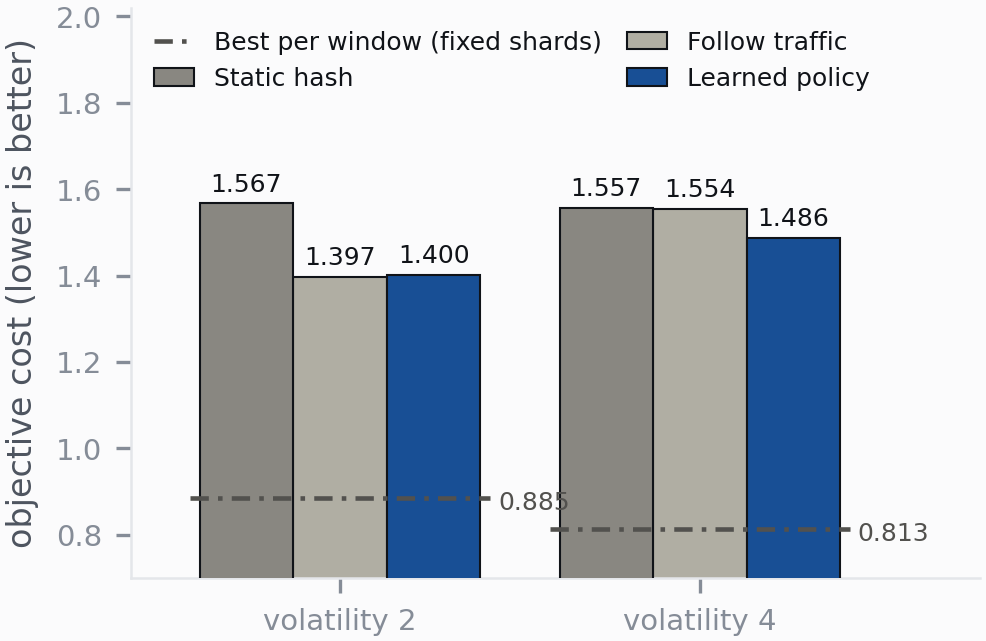
\includegraphics[width=\columnwidth]{objective.png}
\caption{Every policy scored on the combined cost at $w=0.30$, not on latency
alone. At the fastest drift setting the rule's latency advantage is almost
entirely paid back by the data it moves and the imbalance it leaves, and the
learned policy is below both baselines. The distance still left to the
reference is the honest measure of how much remains to do.}
\label{fig:objective}
\end{figure}

Table~\ref{tab:agent} reports five agent runs on held-out seeds, each scored
against the baselines at that run's own movement weight. Scoring a learned run
against a baseline measured at a different weight compares a policy with a
differently judged opponent, and it is the easiest way to manufacture a win,
so the arithmetic is produced by a script rather than by hand.

The agent beats fixed placement in all five runs. At the fastest drift setting
with $w=0.30$ it also beats the rule, on both training seeds, by 0.068 and
0.031 of combined cost. The way it does so is easy to describe. It reaches
139.91\,ms against the rule's 129.04\,ms, so it is slower, but it moves
62.7\,GB against 1086.5\,GB and holds imbalance at 0.776 against 1.003. It is
buying its latency far more cheaply than the rule buys its own.

Fig.~\ref{fig:objective} shows a second result from the same scoring. At the
fastest setting the rule and fixed placement are indistinguishable on the
combined cost, 1.554 against 1.557, even though the rule is 21\,ms faster.
Everything it gains on latency it hands back in movement and imbalance. By
that point the reactive rule has stopped being worth running, which is a
sharper version of the previous subsection's finding than the latency curve
alone can give.
